\documentclass[8pt,aspectratio=169]{beamer}
\usetheme{Madrid}
\usepackage{graphicx}
\usepackage{booktabs}
\usepackage{adjustbox}
\usepackage{multicol}
\usepackage{amsmath}
\usepackage{amssymb}
\usepackage{tikz}
\usepackage{hyperref}
\usepackage{algorithm}
\usepackage{algorithmic}
\usepackage{colortbl}
\usepackage{pgfplots}
\pgfplotsset{compat=1.18}

% TikZ libraries for comics, diagrams, stakeholder maps
\usetikzlibrary{arrows.meta,positioning,shapes.callouts,shapes.geometric,decorations.pathreplacing}

% Color definitions
\definecolor{mlblue}{RGB}{0,102,204}
\definecolor{mlpurple}{RGB}{51,51,178}
\definecolor{mllavender}{RGB}{173,173,224}
\definecolor{mllavender2}{RGB}{193,193,232}
\definecolor{mllavender3}{RGB}{204,204,235}
\definecolor{mllavender4}{RGB}{214,214,239}
\definecolor{mlorange}{RGB}{255, 127, 14}
\definecolor{mlgreen}{RGB}{44, 160, 44}
\definecolor{mlred}{RGB}{214, 39, 40}
\definecolor{mlgray}{RGB}{127, 127, 127}
\definecolor{lightgray}{RGB}{240, 240, 240}
\definecolor{midgray}{RGB}{180, 180, 180}

% NEW COLORS for mini-lecture
\definecolor{dfteal}{RGB}{0,128,128}
\definecolor{dfred}{RGB}{180,30,30}

% Backward compatibility
\colorlet{MLPurple}{mlpurple}
\colorlet{MLBlue}{mlblue}
\colorlet{MLOrange}{mlorange}
\colorlet{MLGreen}{mlgreen}
\colorlet{MLRed}{mlred}
\colorlet{MLLavender}{mllavender}
\colorlet{MLGray}{mlgray}

% Theme colors (exact Madrid settings)
\setbeamercolor{palette primary}{bg=mllavender3,fg=mlpurple}
\setbeamercolor{palette secondary}{bg=mllavender2,fg=mlpurple}
\setbeamercolor{palette tertiary}{bg=mllavender,fg=white}
\setbeamercolor{palette quaternary}{bg=mlpurple,fg=white}
\setbeamercolor{structure}{fg=mlpurple}
\setbeamercolor{section in toc}{fg=mlpurple}
\setbeamercolor{subsection in toc}{fg=mlblue}
\setbeamercolor{title}{fg=mlpurple}
\setbeamercolor{frametitle}{fg=mlpurple,bg=mllavender3}
\setbeamercolor{block title}{bg=mllavender2,fg=mlpurple}
\setbeamercolor{block body}{bg=mllavender4,fg=black}
\setbeamertemplate{navigation symbols}{}
\setbeamertemplate{itemize items}[circle]
\setbeamertemplate{enumerate items}[default]
\setbeamersize{text margin left=5mm,text margin right=5mm}

% Footer
\setbeamertemplate{footline}{
  \leavevmode%
  \hbox{%
    \begin{beamercolorbox}[wd=.333333\paperwidth,ht=2.25ex,dp=1ex,center]{author in head/foot}%
      \usebeamerfont{author in head/foot}Methods and Algorithms
    \end{beamercolorbox}%
    \begin{beamercolorbox}[wd=.333333\paperwidth,ht=2.25ex,dp=1ex,center]{title in head/foot}%
      \usebeamerfont{title in head/foot}MSc Data Science
    \end{beamercolorbox}%
    \begin{beamercolorbox}[wd=.333333\paperwidth,ht=2.25ex,dp=1ex,right]{date in head/foot}%
      \usebeamerfont{date in head/foot}\insertframenumber{} / \inserttotalframenumber\hspace*{2ex}
    \end{beamercolorbox}}%
  \vskip0pt%
}

\newcommand{\bottomnote}[1]{%
\vfill
\vspace{-2mm}
\textcolor{mllavender2}{\rule{\textwidth}{0.4pt}}
\vspace{1mm}
\footnotesize
\textbf{#1}
}

\newenvironment{compactlist}{%
  \begin{itemize}%
    \setlength{\itemsep}{2pt}%
    \setlength{\parskip}{0pt}%
    \setlength{\parsep}{0pt}%
}{%
  \end{itemize}%
}

\newcommand{\highlight}[1]{\textcolor{mlorange}{\textbf{#1}}}
\newcommand{\mathbold}[1]{\boldsymbol{#1}}

\title[Word Embeddings Mini-Lecture]{Word Embeddings}
\subtitle{Mini-Lecture: Teaching Computers to Understand Words}
\author{Methods \& Algorithms}
\date{MSc Data Science -- Spring 2026}

\begin{document}

%% ================================================================
%% SLIDE 1: Title Page
%% ================================================================
\begin{frame}[plain]
\titlepage
\end{frame}

%% ================================================================
%% SLIDE 2: Opening XKCD
%% ================================================================
\begin{frame}[t]{The Machine Learning Pipeline}
\begin{center}
\includegraphics[width=0.6\textwidth,height=0.7\textheight,keepaspectratio]{images/1838_machine_learning.png}
\end{center}

\bottomnote{XKCD \#1838 by Randall Munroe (CC BY-NC 2.5)}
\end{frame}

%% ================================================================
%% SLIDE 3: Words as Vectors
%% ================================================================
\begin{frame}[t]{Words as Vectors: From Symbols to Numbers}
\begin{columns}[T]
\column{0.55\textwidth}
\small
\textbf{The Representation Problem}
\begin{compactlist}
\item Computers need numbers, not words -- how do we encode ``bank'', ``risk'', ``default''?
\item \highlight{One-hot encoding}: each word is a sparse vector with a single 1. Vocabulary of 50k = 50k-dimensional vectors.
\item Problem: one-hot treats ``bank'' and ``finance'' as equally different from ``banana''
\item \highlight{Dense embeddings}: map each word to a short vector (50--300 dims) where similar words are nearby
\end{compactlist}

\begin{block}{Distributional Hypothesis}
\scriptsize ``You shall know a word by the company it keeps'' (Firth, 1957). Words in similar contexts have similar meanings.
\end{block}

\column{0.42\textwidth}
\vspace{2mm}
\footnotesize
\fcolorbox{mlpurple}{mllavender4}{\parbox{0.85\columnwidth}{%
\textbf{One-hot} (sparse, 50k dims):

\vspace{1mm}
\texttt{bank\;= [0,0,1,0,...,0]}

\texttt{risk\;\;= [0,0,0,0,...,1]}

\vspace{2mm}
\textbf{Embedding} (dense, 300 dims):

\vspace{1mm}
\texttt{bank = [0.2, -0.1, ...]}

\texttt{risk\;\;= [0.3, -0.2, ...]}

\vspace{1mm}
\textcolor{mlgreen}{Similar words $\rightarrow$ nearby vectors}
}}
\end{columns}

\bottomnote{Embeddings compress meaning into geometry -- distance = semantic similarity}
\end{frame}

%% ================================================================
%% SLIDE 4: Word2Vec Skip-gram
%% ================================================================
\begin{frame}[t]{Word2Vec: Learning Embeddings from Context}
\begin{columns}[T]
\column{0.55\textwidth}
\small
\textbf{The Skip-gram Model}
\begin{compactlist}
\item Given a center word, predict its surrounding context words
\item Training objective: maximize $P(\text{context} \mid \text{center})$
\item The hidden layer weights become the word embeddings
\item Trained on billions of words of text -- embeddings emerge from co-occurrence patterns
\end{compactlist}

\vspace{1mm}
\scriptsize Example: ``The \underline{bank} reported strong quarterly \underline{earnings}'' -- ``bank'' and ``earnings'' become neighbors in embedding space.

\begin{block}{Insight}
\scriptsize Word2Vec does not understand language -- it learns statistical co-occurrence. But this is enough to capture remarkable semantic structure.
\end{block}

\column{0.42\textwidth}
\vspace{2mm}
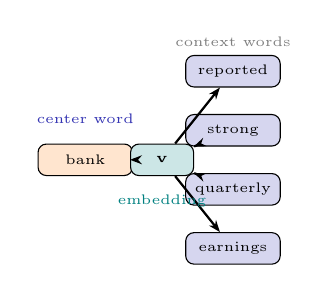
\begin{tikzpicture}[scale=0.75,
  wordnode/.style={draw, rounded corners=3pt, font=\tiny, minimum width=1.2cm, minimum height=0.4cm, align=center}]
% Input
\node[wordnode, fill=mlorange!20] (center) at (1.5,2.5) {bank};
% Context words
\node[wordnode, fill=mllavender4] (c1) at (4.0,4.0) {reported};
\node[wordnode, fill=mllavender4] (c2) at (4.0,3.0) {strong};
\node[wordnode, fill=mllavender4] (c3) at (4.0,2.0) {quarterly};
\node[wordnode, fill=mllavender4] (c4) at (4.0,1.0) {earnings};
% Hidden layer
\node[wordnode, fill=dfteal!20, minimum width=0.8cm] (h) at (2.8,2.5) {$\mathbf{v}$};
% Arrows
\draw[-{Stealth[length=1.5mm]}, thick] (center) -- (h);
\draw[-{Stealth[length=1.5mm]}, thick] (h) -- (c1);
\draw[-{Stealth[length=1.5mm]}, thick] (h) -- (c2);
\draw[-{Stealth[length=1.5mm]}, thick] (h) -- (c3);
\draw[-{Stealth[length=1.5mm]}, thick] (h) -- (c4);
% Labels
\node[font=\tiny, mlpurple] at (1.5,3.2) {center word};
\node[font=\tiny, dfteal] at (2.8,1.8) {embedding};
\node[font=\tiny, mlgray] at (4.0,4.5) {context words};
\end{tikzpicture}
\end{columns}

\bottomnote{Word2Vec (Mikolov et al., 2013) trained on Google News: 100 billion words, 3 million word vectors}
\end{frame}

%% ================================================================
%% SLIDE 5: Semantic Similarity
%% ================================================================
\begin{frame}[t]{Semantic Similarity: Words That Cluster Together}
\begin{columns}[T]
\column{0.55\textwidth}
\small
\textbf{Measuring Word Similarity}
\begin{compactlist}
\item \highlight{Cosine similarity}: $\cos(\mathbf{u}, \mathbf{v}) = \frac{\mathbf{u} \cdot \mathbf{v}}{\|\mathbf{u}\| \|\mathbf{v}\|}$
\item Range: $-1$ (opposite) to $+1$ (identical meaning)
\item Finance words cluster: ``stock'', ``equity'', ``shares'' are neighbors
\item Unrelated words are distant: ``stock'' vs ``elephant''
\end{compactlist}

\begin{block}{Insight}
\scriptsize Cosine similarity ignores vector magnitude -- it measures direction only. Two documents about finance point the same way, regardless of length.
\end{block}

\column{0.42\textwidth}
\vspace{2mm}
\includegraphics[width=0.55\textwidth]{01_word_embedding_space/chart.pdf}
\end{columns}

\bottomnote{In embedding space, semantic relationships become geometric relationships -- similarity = proximity}
\end{frame}

%% ================================================================
%% SLIDE 6: Word Analogies
%% ================================================================
\begin{frame}[t]{Word Analogies: Vector Arithmetic on Meaning}
\begin{columns}[T]
\column{0.55\textwidth}
\small
\textbf{The Famous Analogy Test}
\begin{compactlist}
\item $\vec{\text{king}} - \vec{\text{man}} + \vec{\text{woman}} \approx \vec{\text{queen}}$
\item The ``gender direction'' is captured as a consistent vector offset
\item Finance analogies work too: $\vec{\text{stock}} - \vec{\text{equity}} + \vec{\text{debt}} \approx \vec{\text{bond}}$
\end{compactlist}

\vspace{2mm}
\begin{block}{Insight}
\scriptsize Analogies reveal that embeddings encode relational structure, not just similarity. The same vector offset maps ``man:woman'' as ``king:queen''.
\end{block}

\column{0.42\textwidth}
\vspace{4mm}
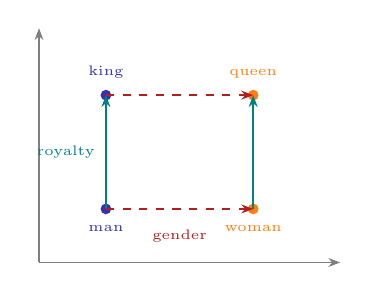
\begin{tikzpicture}[scale=0.85]
% Axes
\draw[-{Stealth[length=1.5mm]}, mlgray] (0,0) -- (4.5,0);
\draw[-{Stealth[length=1.5mm]}, mlgray] (0,0) -- (0,3.5);
% Points
\fill[mlpurple] (1.0,0.8) circle (0.08); \node[font=\tiny, mlpurple, below] at (1.0,0.7) {man};
\fill[mlpurple] (1.0,2.5) circle (0.08); \node[font=\tiny, mlpurple, above] at (1.0,2.6) {king};
\fill[mlorange] (3.2,0.8) circle (0.08); \node[font=\tiny, mlorange, below] at (3.2,0.7) {woman};
\fill[mlorange] (3.2,2.5) circle (0.08); \node[font=\tiny, mlorange, above] at (3.2,2.6) {queen};
% Arrows
\draw[-{Stealth[length=1.5mm]}, dfteal, thick] (1.0,0.8) -- (1.0,2.5);
\draw[-{Stealth[length=1.5mm]}, dfteal, thick] (3.2,0.8) -- (3.2,2.5);
\draw[-{Stealth[length=1.5mm]}, dfred, thick, dashed] (1.0,0.8) -- (3.2,0.8);
\draw[-{Stealth[length=1.5mm]}, dfred, thick, dashed] (1.0,2.5) -- (3.2,2.5);
% Labels
\node[font=\tiny, dfteal] at (0.4,1.65) {royalty};
\node[font=\tiny, dfred] at (2.1,0.4) {gender};
\end{tikzpicture}
\end{columns}

\bottomnote{Analogy accuracy is a standard benchmark for embedding quality -- good embeddings score 60--75\% on the Google analogy test}
\end{frame}

%% ================================================================
%% SLIDE 7: Similarity Heatmap
%% ================================================================
\begin{frame}[t]{Cosine Similarity Between Finance Words}
\begin{columns}[T]
\column{0.55\textwidth}
\small
\textbf{Similarity Heatmap}
\begin{compactlist}
\item Real cosine similarities from pre-trained Word2Vec
\item Finance terms cluster by semantic field: risk words together, asset words together
\item Cross-domain pairs (e.g., ``volatility'' vs ``dividend'') show moderate similarity
\item This structure enables document classification without labeled data
\end{compactlist}

\begin{block}{Insight}
\scriptsize The heatmap reveals that embeddings capture domain-specific structure -- finance words form a coherent subspace.
\end{block}

\column{0.42\textwidth}
\vspace{2mm}
\includegraphics[width=0.55\textwidth]{02_similarity_heatmap/chart.pdf}
\end{columns}

\bottomnote{Pre-trained embeddings transfer knowledge from general text to domain-specific tasks -- fine-tuning adapts them further}
\end{frame}

%% ================================================================
%% SLIDE 8: Pre-trained Models
%% ================================================================
\begin{frame}[t]{Pre-trained Models: Standing on the Shoulders of Giants}
\begin{columns}[T]
\column{0.95\textwidth}
\small
\textbf{From Static to Contextual Embeddings}

\vspace{2mm}
\footnotesize
\begin{tabular}{@{}l c c c@{}}
\toprule
\textbf{Model} & \textbf{Type} & \textbf{Dimensions} & \textbf{Key Feature} \\
\midrule
\rowcolor{mllavender4}
Word2Vec & Static & 100--300 & Fast, simple, one vector per word \\
GloVe & Static & 50--300 & Global co-occurrence statistics \\
\rowcolor{mllavender4}
ELMo & Contextual & 1024 & Different vector per context \\
BERT & Contextual & 768 & Bidirectional, fine-tunable \\
\bottomrule
\end{tabular}

\vspace{3mm}
\begin{compactlist}
\item \highlight{Static}: ``bank'' has ONE vector regardless of context (river bank vs investment bank)
\item \highlight{Contextual}: ``bank'' gets different vectors depending on surrounding words
\item For most finance NLP tasks, fine-tuned BERT outperforms static embeddings
\end{compactlist}
\end{columns}

\bottomnote{FinBERT (Araci, 2019) is BERT fine-tuned on financial text -- state of the art for financial sentiment analysis}
\end{frame}

%% ================================================================
%% SLIDE 9: Finance Application
%% ================================================================
\begin{frame}[t]{Finance Application: NLP for Financial Text}
\begin{columns}[T]
\column{0.55\textwidth}
\small
\textbf{Where Embeddings Meet Finance}
\begin{compactlist}
\item \highlight{Sentiment analysis}: classify earnings calls, news, analyst reports as positive/negative/neutral
\item \highlight{Document similarity}: find SEC filings similar to a reference document using cosine similarity of averaged embeddings
\item \highlight{ESG scoring}: embed company reports and measure proximity to ESG-related concept vectors
\end{compactlist}

\begin{block}{Insight}
\scriptsize Embeddings turn unstructured text into structured features. Once text is a vector, any ML algorithm can process it.
\end{block}

\column{0.42\textwidth}
\vspace{2mm}
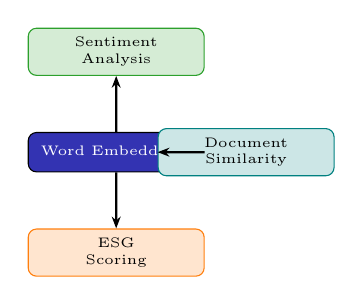
\begin{tikzpicture}[scale=0.75,
  appnode/.style={draw, rounded corners=3pt, font=\tiny, text width=2.0cm, align=center, minimum height=0.5cm}]
% Center: Embeddings
\node[appnode, fill=mlpurple, text=white] (emb) at (2.0,2.5) {Word Embeddings};
% Applications
\node[appnode, fill=mlgreen!20, draw=mlgreen] (sent) at (2.0,4.2) {Sentiment\\Analysis};
\node[appnode, fill=dfteal!20, draw=dfteal] (sim) at (4.2,2.5) {Document\\Similarity};
\node[appnode, fill=mlorange!20, draw=mlorange] (esg) at (2.0,0.8) {ESG\\Scoring};
% Arrows
\draw[-{Stealth[length=1.5mm]}, thick] (emb) -- (sent);
\draw[-{Stealth[length=1.5mm]}, thick] (emb) -- (sim);
\draw[-{Stealth[length=1.5mm]}, thick] (emb) -- (esg);
\end{tikzpicture}
\end{columns}

\bottomnote{Loughran \& McDonald (2011) showed that general-purpose sentiment lexicons fail on financial text -- domain-specific embeddings fix this}
\end{frame}

%% ================================================================
%% SLIDE 10: Summary
%% ================================================================
\begin{frame}[t]{Summary: Word Embeddings in 4 Takeaways}
\begin{columns}[T]
\column{0.95\textwidth}
\small
\begin{enumerate}
\setlength{\itemsep}{6pt}
\item \highlight{Representation}: Dense embeddings map words to short vectors where semantic similarity = geometric proximity, replacing sparse one-hot encoding
\item \highlight{Word2Vec}: Skip-gram learns embeddings by predicting context words -- co-occurrence statistics produce semantic structure
\item \highlight{Analogies}: Vector arithmetic captures relational meaning (king $-$ man $+$ woman $=$ queen), enabling zero-shot reasoning
\item \highlight{Finance}: Embeddings power sentiment analysis, document similarity, and ESG scoring -- turning unstructured text into ML-ready features
\end{enumerate}

\vspace{4mm}
\begin{block}{Next Steps}
\scriptsize Explore the deep dive slides for negative sampling, GloVe derivation, and contextual embeddings. Try the notebook to train Word2Vec on financial news.
\end{block}
\end{columns}

\bottomnote{Embeddings are the bridge between human language and machine learning -- the foundation of modern NLP}
\end{frame}

\end{document}
